\documentclass[10pt,landscape,a4paper]{article}
\usepackage[utf8]{inputenc}
\usepackage[ngerman]{babel}
\usepackage[T1]{fontenc}
%\usepackage[LY1,T1]{fontenc}
%\usepackage{frutigernext}
%\usepackage[lf,minionint]{MinionPro}
\usepackage{tikz}
\usetikzlibrary{shapes,positioning,arrows,fit,calc,graphs,graphs.standard}
\usepackage[nosf]{kpfonts}
\usepackage[t1]{sourcesanspro}
\usepackage{multicol}
\usepackage{wrapfig}
\usepackage[top=0mm,bottom=1mm,left=0mm,right=1mm]{geometry}
\usepackage[framemethod=tikz]{mdframed}
\usepackage{microtype}
\usepackage{pdfpages}
\usepackage{graphicx}

\let\bar\overline
% \everydisplay\expandafter{\the\everydisplay \setlength{\abovedisplayskip}{2pt} \setlength{\belowdisplayskip}{2pt}}
\setlength{\abovedisplayskip}{1pt} % Space above equations
\setlength{\belowdisplayskip}{1pt} % Space below equations
\setlength{\abovedisplayshortskip}{1pt} % Space above equations if the preceding line is short
\setlength{\belowdisplayshortskip}{1pt} % Space below equations if the following line is short

\definecolor{myblue}{cmyk}{1,.72,0,.38}

\def\firstcircle{(0,0) circle (1.5cm)}
\def\secondcircle{(0:2cm) circle (1.5cm)}

\colorlet{circle edge}{myblue}
\colorlet{circle area}{myblue!5}

\tikzset{filled/.style={fill=circle area, draw=circle edge, thick},
    outline/.style={draw=circle edge, thick}}
    
\pgfdeclarelayer{background}
\pgfsetlayers{background,main}

\everymath\expandafter{\the\everymath \color{myblue}}
\everydisplay\expandafter{\the\everydisplay \color{myblue}}

\renewcommand{\baselinestretch}{.8}
\pagestyle{empty}

\global\mdfdefinestyle{header}{%
linecolor=gray,linewidth=1pt,%
leftmargin=0mm,rightmargin=0mm,skipbelow=0mm,skipabove=0mm,
}

\newcommand{\header}{
\begin{mdframed}[style=header]
\footnotesize
\sffamily
Hilfszettel zur Klausur\\
von~Tim~S.,~Seite~\thepage~von~2
\end{mdframed}
}

\makeatletter % Author: https://tex.stackexchange.com/questions/218587/how-to-set-one-header-for-each-page-using-multicols
\renewcommand{\section}{\@startsection{section}{1}{0mm}%
                                {.2ex}%
                                {.2ex}%x
                                {\color{myblue}\sffamily\small\bfseries}}
\renewcommand{\subsection}{\@startsection{subsection}{1}{0mm}%
                                {.2ex}%
                                {.2ex}%x
                                {\sffamily\bfseries}}



\def\multi@column@out{%
   \ifnum\outputpenalty <-\@M
   \speci@ls \else
   \ifvoid\colbreak@box\else
     \mult@info\@ne{Re-adding forced
               break(s) for splitting}%
     \setbox\@cclv\vbox{%
        \unvbox\colbreak@box
        \penalty-\@Mv\unvbox\@cclv}%
   \fi
   \splittopskip\topskip
   \splitmaxdepth\maxdepth
   \dimen@\@colroom
   \divide\skip\footins\col@number
   \ifvoid\footins \else
      \leave@mult@footins
   \fi
   \let\ifshr@kingsaved\ifshr@king
   \ifvbox \@kludgeins
     \advance \dimen@ -\ht\@kludgeins
     \ifdim \wd\@kludgeins>\z@
        \shr@nkingtrue
     \fi
   \fi
   \process@cols\mult@gfirstbox{%
%%%%% START CHANGE
\ifnum\count@=\numexpr\mult@rightbox+2\relax
          \setbox\count@\vsplit\@cclv to \dimexpr \dimen@-1cm\relax
% \setbox\count@\vbox to \dimen@{\vbox to 1cm{\header}\unvbox\count@\vss}%
\else
      \setbox\count@\vsplit\@cclv to \dimen@
\fi
%%%%% END CHANGE
            \set@keptmarks
            \setbox\count@
                 \vbox to\dimen@
                  {\unvbox\count@
                   \remove@discardable@items
                   \ifshr@nking\vfill\fi}%
           }%
   \setbox\mult@rightbox
       \vsplit\@cclv to\dimen@
   \set@keptmarks
   \setbox\mult@rightbox\vbox to\dimen@
          {\unvbox\mult@rightbox
           \remove@discardable@items
           \ifshr@nking\vfill\fi}%
   \let\ifshr@king\ifshr@kingsaved
   \ifvoid\@cclv \else
       \unvbox\@cclv
       \ifnum\outputpenalty=\@M
       \else
          \penalty\outputpenalty
       \fi
       \ifvoid\footins\else
         \PackageWarning{multicol}%
          {I moved some lines to
           the next page.\MessageBreak
           Footnotes on page
           \thepage\space might be wrong}%
       \fi
       \ifnum \c@tracingmulticols>\thr@@
                    \hrule\allowbreak \fi
   \fi
   \ifx\@empty\kept@firstmark
      \let\firstmark\kept@topmark
      \let\botmark\kept@topmark
   \else
      \let\firstmark\kept@firstmark
      \let\botmark\kept@botmark
   \fi
   \let\topmark\kept@topmark
   \mult@info\tw@
        {Use kept top mark:\MessageBreak
          \meaning\kept@topmark
         \MessageBreak
         Use kept first mark:\MessageBreak
          \meaning\kept@firstmark
        \MessageBreak
         Use kept bot mark:\MessageBreak
          \meaning\kept@botmark
        \MessageBreak
         Produce first mark:\MessageBreak
          \meaning\firstmark
        \MessageBreak
        Produce bot mark:\MessageBreak
          \meaning\botmark
         \@gobbletwo}%
   \setbox\@cclv\vbox{\unvbox\partial@page
                      \page@sofar}%
   \@makecol\@outputpage
     \global\let\kept@topmark\botmark
     \global\let\kept@firstmark\@empty
     \global\let\kept@botmark\@empty
     \mult@info\tw@
        {(Re)Init top mark:\MessageBreak
         \meaning\kept@topmark
         \@gobbletwo}%
   \global\@colroom\@colht
   \global \@mparbottom \z@
   \process@deferreds
   \@whilesw\if@fcolmade\fi{\@outputpage
      \global\@colroom\@colht
      \process@deferreds}%
   \mult@info\@ne
     {Colroom:\MessageBreak
      \the\@colht\space
              after float space removed
              = \the\@colroom \@gobble}%
    \set@mult@vsize \global
  \fi}

\makeatother
\setlength{\parindent}{0pt}


\begin{document}
%\footnotesize
\small
\begin{multicols*}{5}
\section{Light \& color}
\subsection*{Light}
refraction(transparent obj) \\
absorbing \& reflection (opaque obj)
\subsection*{color perception}
dependencies: \\
1. color of lights: physics of light \& reflectance of the surface. \\
2. percieved colors: visual system receptor, lights..


\section{Image filtering}
\subsection*{Digital Image formation}
1. Formation of image: illumination + scene element + imaging system + image plane\\
2. Digital camera: sample 2d space on regular grid \& quantize each sample (round to nearest integer)
\subsection*{Image noise, filtering, conv}
1. \textbf{common types of noise}: salt/pepper noise, impulse noise (random occurrences of white pixels), Guassian noise\\
2. \textbf{Cross correlation} filtering $G=H\otimes F$: \\
$G[i,j] = \sum_{u=-k}^{k} \sum_{v=-k}^{k} H[u, v] F[i+u, j+v]$ \\
\textbf{Convolution} (cross correlation will flip the img):\\
$G[i,j] = \sum_{u=-k}^{k} \sum_{v=-k}^{k} H[u, v] F[i-u, j-v]$\\
box filter, \quad Gaussian filter:
\[
 \frac{1}{9}
\begin{bmatrix}
 1 & 1&1 \\
 1&?&1 \\
 1&1&1
\end{bmatrix}, \quad
\frac{1}{16}
\begin{bmatrix}
 1&2&1 \\
 2&4&2 \\
 1&2&1
\end{bmatrix}
\]
3. Runtime complexity: 
$O(C_{in} \cdot C_{out} \cdot N^2 \cdot M^2)
$ \\
4. Separability:  
$1D gs * 1D gs = 2D gs$\\
$Image * 2D gs = Image * 1D gs * 1D gs$
5. Smoothing: remove high-freq components (low pass filter) \\
6. Prop of convs:\\
a. Commutative: f*g = g*f \\
b. Associative: (f*g)*h = f*(g*h) \\
c. Distributive over +: l*(f1+f2) = l*f1+l*f2 \\
d. Shift invariant shift(l*f) = shift(l)*f \\
7. \textbf{Sharpening filter} (image - smoothed =  details):
positive in the middle \& negative around \\
7. \textbf{Nonlinear filter}: median filter \\
9.\textbf{ hybrid image}: 
Laplacian filter(identify rapid change) ~ unit impulse - Gaussian
\[
\mathbf{K} = 
\begin{bmatrix}
0 & -1 & 0 \\
-1 & 4 & -1 \\
0 & -1 & 0
\end{bmatrix}
\]

\section{Edge detection}
% \subsection*{What Causes an Edge?}
% \begin{itemize}
%     \item \textbf{Depth discontinuity}: Object boundaries.
%     \item \textbf{Surface orientation changes}: Shape variations.
%     \item \textbf{Cast shadows}: Lighting effects.
%     \item \textbf{Reflectance change}: Differences in texture or material appearance.
% \end{itemize}

\subsection*{Derivatives and Gradients}
% \textbf{First derivative:} Detects rapid changes in intensity (edge points align with peaks in derivative). 

\textbf{Image Gradient:} Measures the rate and direction of intensity change. 

\textbf{Gradient Magnitude/Direction (Edge Strength/Orientation)}
\[
|\nabla I| = \sqrt{\left(\frac{\partial I}{\partial x}\right)^2 + \left(\frac{\partial I}{\partial y}\right)^2},
\quad
\theta = \tan^{-1}\left(\frac{\partial I / \partial y}{\partial I / \partial x}\right)
\]

% \textbf{Gradient Direction (Orientation)}
% \[
% \theta = \tan^{-1}\left(\frac{\partial I / \partial y}{\partial I / \partial x}\right)
% \]

\subsection*{Edge Detection Filters}
\textbf{Sobel Filter:} compute gradients.
\[
\text{Horizontal} = 
\begin{bmatrix}
-1 & 0 & 1 \\
-2 & 0 & 2 \\
-1 & 0 & 1
\end{bmatrix}
% \quad
% \text{Vertical} = 
% \begin{bmatrix}
% -1 & -2 & -1 \\
% 0 & 0 & 0 \\
% 1 & 2 & 1
% \end{bmatrix}
\]

\textbf{Prewitt Filter:} Change 2 in Sobel to 1 for noise robustness.
% \[
% \text{Horizontal} = 
% \begin{bmatrix}
% -1 & 0 & 1 \\
% -1 & 0 & 1 \\
% -1 & 0 & 1
% \end{bmatrix}
% \quad
% \text{Vertical} = 
% \begin{bmatrix}
% -1 & -1 & -1 \\
% 0 & 0 & 0 \\
% 1 & 1 & 1
% \end{bmatrix}
% \]
\subsection*{Canny Edge Detection Steps}
1. \textbf{Smoothing}: w a Gaussian filter.\\
2. \textbf{Gradient Calculation}: Compute gradients w Sobel filters.\\
3. \textbf{Non-Maximum Suppression}: Retain local maxima along the grad direction to thin the edges.\\
% 4. \textbf{Hysteresis Thresholding}: A \textbf{high thres} to start edges and a \textbf{low thres} to continue edges.
4. \textbf{Thresholding}: A \textbf{high thres} to start edges and a \textbf{low thres} to continue edges.

\section{Local Feature Detection}

\subsection*{Desired Properties of Local Features}
1. \textbf{Repeatability}: Detectable across images despite transformations.\\
2. \textbf{Saliency}: Be distinct. \\
3. \textbf{Efficiency}: Lighter than total pixels. \\
4. \textbf{Locality}: Cover small, clutter-resistant regions.


\subsection*{Corners as Interest Points}
1. \textbf{Flat Region}: No intensity change in any direction. \\
2. \textbf{Edge}: No change along the edge direction. \\
3. \textbf{Corner}: Large change in all directions.
\subsection*{Harris Corner Detector}
Invariant to rotation, not scale\\
1. \textbf{Compute $M$} for each image window:
    \[
    M = 
    \begin{bmatrix}
    \sum I_x^2 & \sum I_x I_y \\
    \sum I_x I_y & \sum I_y^2
    \end{bmatrix}
    \] \\
2. \textbf{Corner Response Function}:
    \[
    R = \det(M) - \alpha \cdot (\text{trace}(M))^2
    \] \\
3. \textbf{Thresholding}: Retain points with large $R$ values. \\
4. \textbf{Non-Maximum Suppression}: Keep local maxima to avoid redundant corners.

\subsection*{Blob Detection and Scale Selection}
1. Scale-invariant but not rotation.\\
2. \textbf{Laplacian of Gaussian (LoG)}:
    \[
    \nabla^2 G = \frac{\partial^2 G}{\partial x^2} + \frac{\partial^2 G}{\partial y^2}
    \]
3. \textbf{Characteristic Scale}: Scale at which the LoG response is maximized.

\subsection*{Feature Matching}
1. Extract keypoint features.\\
2. Compute potential matches between images.\\
3. Hypothesize transformation $T$ to align related matches.\\
4. Verify transformation by checking for consistency across matches.


\section{Local Feature Description}

% \subsection*{Local Feature Detection and Description}
% 1. Detection: Identify interest points using methods like the Harris Corner Detector or Blob Detector. \\
% 2. Description: Extract vector feature descriptors surrounding each interest point. \\
% 3. Matching: Determine correspondences between descriptors in different views.

\subsection*{SIFT Descriptor (Lowe, 2004)}
1. Compute gradients within sub-patches --> histograms of gradient orientations. \\
2. Rotate the patch based on dominant gradient --> rotation invariance. \\
3. Map pixels to a 128-dimensional vec. \\
4. Invariance to scale and rotation, partial invariance to illumination changes, capable of handling occlusion.

\subsection*{Blob Detection and Difference of Gaussians (DoG)}
1. Key: identifying maxima or minima in both position and scale. \\
2. The Laplacian of Gaussian (LoG) can be approximated with DoG for better efficiency:
   \[
   \text{DoG}(x, y, \sigma) = G(x, y, k\sigma) - G(x, y, \sigma)
   \]
3. The characteristic scale corresponds to the peak LoG response, capturing feature blobs across multiple scales.

\subsection*{Matching Techniques}
1. Compute candidate matches w Sum of Squared Distances (SSD) etc. \\
2. Use Nearest Neighbor Search with a thres of nearest to second-nearest descriptor. \\
   \[
   \text{Ratio} = \frac{\text{Distance to best match}}{\text{Distance to second-best match}}
   \]
   If the ratio is low, the match is reliable; if high, it may indicate ambiguity.

% \subsection*{Applications of Local Invariant Features}
% 1. Wide baseline stereo matching. \\
% 2. Motion tracking and panoramas. \\
% 3. Mobile robot navigation and 3D reconstruction. \\
% 4. Object and scene recognition.


\section{Fitting and Hough Transform}
% 1. Goal: Find the best parametric model (e.g., line, circle) to represent a set of features in images, despite noise, missing parts, or clutter. \\
% 2. Challenges in Line Fitting: \\
%    - Extra edge points (clutter) may not belong to any line. \\
%    - Incomplete lines must be bridged from partial evidence. \\
%    - Noise in edge points and orientations complicates accurate fitting. \\

\subsection*{Hough Transform for Line Detection}
% 1. Concept: Use a \textbf{voting mechanism} to let each feature vote for possible model parameters.  \\
1. Mapping to Hough Space: \\
   - \textbf{Image space} $(x, y)$: Holds edge points. \\
   - \textbf{Hough space} $(m, b)$: Lines $y = mx + b$. \\
   - A point in the image space --> a line in Hough space. \\
2. Advantages: robust to noise, tolerance to disconnected segments
\subsection*{Hough Transform Algorithm (Line Detection)}
1. Initialize accumulator arr $H[m, b] = 0$. \\
2. For each edge point $(x, y)$ in the image: \\
   \null \quad For each possible slope $m$: \\
   \null \quad \quad Calculate $b = y - mx$. \\
   \null \quad \quad Increment $H[m, b]$ by 1. \\
3. Find the $(m, b)$ with the highest votes in $H$. \\
% 4. The detected lines correspond to the parameters with maximum votes.

\subsection*{Polar Representation of Lines}
1. To avoid infinite slopes for vertical lines, use the polar equation: \\
   \[
   x \cos \theta + y \sin \theta = d
   \]
   % where $d$ is the perpendicular distance from the origin, and $\theta$ is the angle between the x-axis and the perpendicular to the line. \\
2. Each edge point votes for a sinusoid in $(d, \theta)$ space, and intersections correspond to lines in the original image space.
\subsection*{Extensions of Hough Transform}
- Use gradient direction to reduce param search. \\
- Assign higher weights to stronger edges during voting. \\
- Adapt the transform for circles etc. \\

% \subsection*{Extensions and Applications}
% 1. Extensions: \\
%    - Use gradient direction to reduce parameter search. \\
%    - Assign higher weights to stronger edges during voting. \\
%    - Adapt the transform for circles or other shapes. \\
% 2. Applications: \\
%    - Line and circle detection in images. \\
%    - Iris detection and coin recognition. \\
%    - Generalized Hough Transform for arbitrary shape matching.

\subsection*{Pros and Cons of Hough Transform}
1. \textbf{Pros:} \\
   - Can handle occlusion, noise, and gaps in features. \\
   - Detects multiple instances of a model in a single pass. \\
2. \textbf{Cons:} \\
   - Search time increases exponentially with more parameters. \\
   - Non-target shapes may produce spurious peaks. \\
   - Requires careful choice of grid size for parameter space.

\section{Fitting a 2D Transformation}
% 1. Given two images, the goal is to learn a transformation \(T\) that aligns them. \\
% 2. Transformation \(T\) can be fit using matching feature pairs called correspondences. \\

\subsection*{Parametric Warping}
1. Transformation \(T\) can take different forms: \\
   - Translation, Rotation, Scaling, Affine, and Perspective. \\
2. These transformations can be represented as matrix operations, such as:
   \[
   \mathbf{p'} = \mathbf{T} \cdot \mathbf{p}
   \]
   % where \(\mathbf{p} = (x, y)\) and \(\mathbf{p'} = (x', y')\) are points in the original and transformed space.

\subsection*{Basic Transformations as Matrices}
1. \textbf{Scaling}, \quad \textbf{Rotation}: \\
   \[
   \mathbf{S} = 
   \begin{bmatrix}
   s_x & 0 \\
   0 & s_y
   \end{bmatrix}, \quad
   \mathbf{R} =
   \begin{bmatrix}
   \cos \theta & -\sin \theta \\
   \sin \theta & \cos \theta
   \end{bmatrix}
   \] 
2. \textbf{Shear}, \quad \textbf{Translation}: \\
   \[
   \mathbf{S} = 
   \begin{bmatrix}
   1 & \alpha \\
   \beta & 1
   \end{bmatrix}, \quad
   \mathbf{T} =
   \begin{bmatrix}
   1 & 0 & t_x \\
   0 & 1 & t_y \\
   0 & 0 & 1
   \end{bmatrix}
   \]

\subsection*{Affine Transformations}
1. Combine linear transformations (scaling, rotation, shear) and translation:
   \[
   \mathbf{A} =
   \begin{bmatrix}
   a_{11} & a_{12} & t_x \\
   a_{21} & a_{22} & t_y \\
   0 & 0 & 1
   \end{bmatrix}
   \]
2. Parallel lines remain parallel under affine transformations.

\subsection*{Using RANSAC for Robust Fitting}
1. RANSAC (Random Sample Consensus):
   - Randomly select a set of pts, estimate the transformation. \\
   - Compute the transformation and identify inliers. \\
   - If enough inliers, recompute the transformation with all inliers. \\
2. Keep the transformation with the most inliers across multiple trials.

\subsection*{Summary of RANSAC}
1. \textbf{Pros}: \\
   - Robust to noise \& outliers(extremely x). \\
   % - Works well for a variety of problems. \\
2. \textbf{Cons}: \\
   - Requires careful tuning of hyperparams. \\
   - Perf drops with low inlier ratios. \\
   - Can struggle with poor initialization based on minimum samples.

\section{Homography and Image Mosaics}
1. \textbf{Goal:} Use homography to align and stitch images into a seamless mosaic. \\
2. \textbf{Homography:} A projective transformation that maps points from one image plane to another. \\
   % - Allows mapping of rectangles to quadrilaterals and preserves straight lines (not necessarily parallel lines). \\
   - Preserve straight lines, not necessarily parallel lines/length/angle. \\
   - Represented by a 3x3 matrix \(H\):
   \[
   \mathbf{p'} = H \cdot \mathbf{p}
   \]
   % where \(\mathbf{p}\) and \(\mathbf{p'}\) are homogeneous coordinates of corresponding points in two images.

\subsection*{Generating Image Mosaics}
1. Capture a sequence of images from the same camera position. \\
2. Compute the transformation between consecutive images w feature-based alignment. \\
3. Use homography to transform and align images. \\
4. Blend aligned images to create the final mosaic. \\
% 5. Repeat for additional images to extend the mosaic.

\subsection*{Image Warping and Reprojection}
1. \textbf{Forward Warping:} 
% Map each pixel in the source image to a new position:
   \[
   (x', y') = T(x, y)
   \]
   - If a pixel lands between two pixels in the target image, distribute its color among neighbors (splatting). \\
2. \textbf{Inverse Warping:} 
% Compute the source pixel for each target pixel using the inverse transformation:
   \[
   (x, y) = T^{-1}(x', y')
   \]
   - Interpolate color values from neighbors (e.g., nearest neighbor, bilinear interpolation).

\subsection*{RANSAC for Homography Estimation}
1. Randomly select 4 pairs of corresponding pts. \\
2. Compute the homography matrix \(H\). \\
3. Identify inliers—pairs that satisfy:
   \[
   \text{SSD}(\mathbf{p'}, H \cdot \mathbf{p}) < \epsilon
   \]
4. Keep the set of inliers w the largest size. \\
5. Recompute \(H\) using all inliers w least squares.

% \subsection*{Applications of Homography}
% 1. \textbf{Image Mosaics:} Stitch images to create panoramic views. \\
% 2. \textbf{Image Rectification:} Align images to correct geometric distortions. \\
% 3. \textbf{Virtual Views:} Synthesize new viewpoints using homography and image warping.

% \subsection*{Summary of Alignment and Warping}
% 1. Write 2D transformations as matrix-vector multiplication. \\
% 2. Use homogeneous coordinates to handle translations. \\
% 3. Perform image warping using forward or inverse mapping. \\
% 4. Fit transformations by solving for unknown parameters using corresponding points. \\
% 5. Create mosaics by warping and stitching images aligned by homography.

\section{Image Formation}
% 1. \textbf{Image Formation:} Capturing real-world objects into an image involves physical, geometric, and optical parameters. \\

\subsection*{Physical Parameters}
1. \textbf{Photometric:} 
   - Type, direction, and intensity of light reaching the sensor. \\
   - Surface reflectance properties. \\
2. \textbf{Geometric:} 
   - Type of projection (e.g., perspective, orthographic). \\
   - Camera pose and position. \\
3. \textbf{Optical:}
   - Lens type, focal length, aperture, and shutter speed. \\

\subsection*{Pinhole Camera Model}
1. A camera model where light passes through a pinhole onto a film/sensor. \\
- Reduces blurring by blocking most light rays and allows sharp image formation. \\

\subsection*{Projective Geometry}
1. Projection maps 3D world coordinates to 2D image coordinates. \\
   % - Example: \( u = \frac{f X}{Z} + u_0 \), \( v = \frac{f Y}{Z} + v_0 \). \\
\
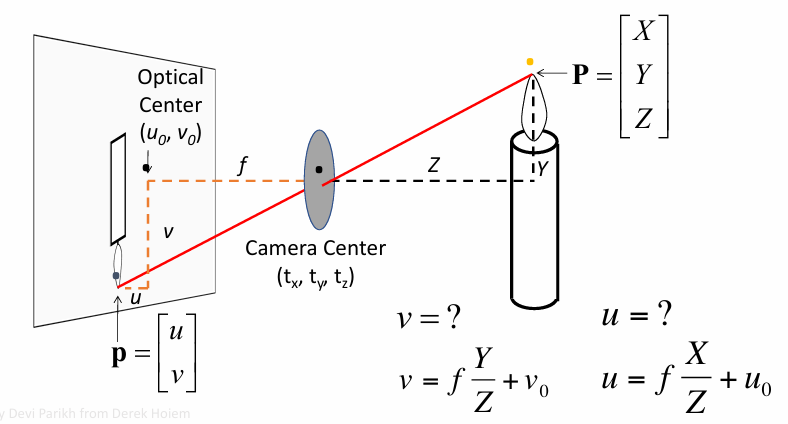
\includegraphics[width=1\linewidth]{images/l10-pinhole.png}
    % \caption{Pinhole Camera Model: Light rays from the object pass through the pinhole, forming an inverted image on the image plane.}
    % \label{fig:pinhole-model}

2. \textbf{Vanishing Points:} 3D Parallel lines -> converge at a point in the image. (Vertical vanishing point: infinity)\\
\textbf{Vanishing Line:} 3D Parallel lines -> converge at a line in the image.

\subsection*{Homogeneous Coordinates and Camera Matrix}
1. Homogeneous coordinates: add another axis, translation --> mat mul. \\
2. \textbf{Intrinsic Matrix} (\(K\)): Encodes internal camera properties. Deg of freedom: 5
   \[
   K = 
   \begin{bmatrix}
   f_x & s & c_x \\
   0 & f_y & c_y \\
   0 & 0 & 1
   \end{bmatrix}
   \]
   - \(f_x, f_y\): Focal length. \\
   - \(s\): Skew factor (usually 0) to account for non-rectangular pixels. \\
   - \(c_x, c_y\): Optical center coordinates (principal point). \\
3. \textbf{Extrinsic Matrix} (\([R | t]\)): External camera params. Deg of freedom: 6\\
   % \[
   % [R \mid t] = 
   % \begin{bmatrix}
   % R & t \\
   % 0 & 1
   % \end{bmatrix}
   % \]
   \[
   R = R_x(\alpha) R_y(\beta) R_z(\gamma)
   \]
   \[
   R_x(\alpha) = 
   \begin{bmatrix}
   1 & 0 & 0 \\
   0 & \cos \alpha & -\sin \alpha \\
   0 & \sin \alpha & \cos \alpha
   \end{bmatrix}
   % , \quad
   % R_y(\beta) = 
   % \begin{bmatrix}
   % \cos \beta & 0 & \sin \beta \\
   % 0 & 1 & 0 \\
   % -\sin \beta & 0 & \cos \beta
   % \end{bmatrix}, \quad
   % R_z(\gamma) = 
   % \begin{bmatrix}
   % \cos \gamma & -\sin \gamma & 0 \\
   % \sin \gamma & \cos \gamma & 0 \\
   % 0 & 0 & 1
   % \end{bmatrix}
   \]
   % - \(R_x(\alpha)\): Rotation around the x-axis by angle \(\alpha\). \\
   % - \(R_y(\beta)\): Rotation around the y-axis by angle \(\beta\). \\
   % - \(R_z(\gamma)\): Rotation around the z-axis by angle \(\gamma\). \\
   - \(R\), \(t\): from world's coordinate to cam's
   % - \(R\): Rotation matrix representing the camera's orientation relative to the world. \\
   % - \(t\): Translation vector representing the camera’s position. \\

\subsection*{Orthographic and Weak Perspective Proj}
1. \textbf{Orthographic Projection:} The distance to the image plane is infinite. \\
2. \textbf{Weak Perspective:} An approximation where object dimensions are small relative to the camera distance. \\

% \subsection*{Summary}
% 1. Key concepts: \textbf{vanishing points}, \textbf{pinhole camera model}, \textbf{homogeneous coordinates}. \\
% 2. Understanding these models helps explain image formation, projection, and camera calibration.

\section{Stereo and Camera Calibration}
% 1. \textbf{Stereo Vision:} recover the 3D structure of a scene from multiple 2D images. \\
% 2. \textbf{Single-View Limitation:} depth information is ambiguous as each pixel only provides a ray. \\

\subsection*{Stereo Vision}
1. \textbf{Stereo Vision Setup:} Two or more cams capture the scene from slightly different viewpoints. \\
% 2. \textbf{Correspondences:} Matching points (features) in the images are identified to calculate depth. \\
% 3. \textbf{Epipolar Geometry:} A key concept in stereo vision that defines the relationship between two views. \\
2. \textbf{Disparity:} The difference in the position of corresponding pts between the two images. Depth is inversely proportional to disparity:
   \[
   \text{Depth} = \frac{f \cdot B}{\text{Disparity}}
   \]
   where \(f\) is the focal length, and \(B\) is the baseline (distance between the cameras). \\



\subsection*{Projection Matrix and Calibration Process}
\textbf{Projection Model:} 
% 1. The full projection matrix relates world coordinates to image coordinates:
   % \[
   % p = MX, M = K [R | t]
   % \]
   \[
   \mathbf{p} = \lambda M \mathbf{X}
   \]
   where \(M = K [R | t]\), \(3 \times 4\) projection matrix \\
% 1. \textbf{Camera calibration:} Estimates the intrinsic matrix \(K\) and extrinsic parameters \([R | t]\) to convert 3D points to 2D image coordinates.   \\
1. \textbf{Camera calibration:} Estimates M given p, X.   \\
- \textbf{Calibration Targets:} Objects with known dimensions (like checkerboards) \\
% are used to find correspondences and solve for the calibration matrix. \\
- \textbf{Linear Calibration Method:} Uses correspondences between 3D points and their projections to estimate \(M\). \\
   % - \textbf{Projection Model:} 
   %   \[
   %   \mathbf{p} = \lambda M \mathbf{X},
   %   \]
   - \textbf{Linearization via Cross-Product:} The projection model is linearized as:
     \[
     \mathbf{p} \times (M \mathbf{X}) = 0.
     \]
       \[
       \begin{bmatrix}
       u_i \\
       v_i \\
       1
       \end{bmatrix}
       \times
       \begin{bmatrix}
       m_1^T \mathbf{X}_i \\
       m_2^T \mathbf{X}_i \\
       m_3^T \mathbf{X}_i
       \end{bmatrix}
       =
       \begin{bmatrix}
       0 \\
       0 \\
       0
       \end{bmatrix}.
       \]
    \[
   \begin{bmatrix}
       0^T & -\mathbf{X}_i^T & v_i \mathbf{X}_i^T \\
       \mathbf{X}_i^T & 0^T & -u_i \mathbf{X}_i^T \\
       -v_i \mathbf{X}_i^T & u_i \mathbf{X}_i^T & 0^T
       \end{bmatrix}
       \begin{bmatrix}
       m_1 \\
       m_2 \\
       m_3
       \end{bmatrix}
       =
       \begin{bmatrix}
       0 \\
       0 \\
       0
       \end{bmatrix}.
    \]
    \textbf{Note: }2 linearly independent eqs per correspondence, M (3x4) 11 deg of freedom\\
   - \textbf{Stacking Equations:}  For \(n\) correspondences:
      \[
       A \mathbf{m} = 0,
   \]
   where \(A\) is a \(2n \times 12\) matrix and \(\mathbf{m}\) contains 12 unknown entries of \(M\).

   - \textbf{Solving the System:} Use SVD to find the eigenvector of \(A^T A\) corresponding to the smallest eigenvalue, providing an initial estimate of \(M\). \\
   % - \textbf{Refinement with Non-linear Optimization:} A non-linear optimizer (e.g., Levenberg-Marquardt) refines the solution to handle noise and improve accuracy. \\
  - Note: Can use a\textbf{ non-linear optimizer} (e.g., Levenberg-Marquardt) to handle noise and improve accuracy. \\

2. \textbf{Triangulation:} Given M,p --> X\\
% Given multiple images and correspondences, triangulation computes the 3D location of a point by finding the intersection of rays from each camera. \\
   - \textbf{Method 1: Geometric Approach}  
     Find the shortest segment between viewing rays and select the midpoint of this segment. \\
   - \textbf{Method 2: Non-linear Optimization}  
     % Minimize the reprojection error by finding the point \(X\) that minimizes:
     \[
     X = argmin (
     \sum_i d(\mathbf{p}_i, M_i X)^2 ),
     \]
% \subsection*{Summary}
% 1. \textbf{Stereo vision} recovers depth by matching points across multiple images. \\
% 2. \textbf{Camera calibration} finds the intrinsic and extrinsic parameters to project 3D points into 2D. \\
% 3. Understanding these principles is essential for tasks such as depth estimation, 3D reconstruction, and structure from motion.

\section{Epipolar Geometry}
\subsection*{Epipolar Geometry:} Describes the geometric relationship between two cameras and the corresponding points in their images. 
% It provides constraints that simplify 3D reconstruction and stereo matching. 

1. \textbf{Epipoles:} The intersections of the baseline (the line connecting the two camera centers) with the image planes. Each epipole is the projection of the other camera center. \\
   - All epipolar lines for a given image pass through the epipole. \\
   - Image plane parallel: Epipoles infinitely far away, epipolar lines parallel

   
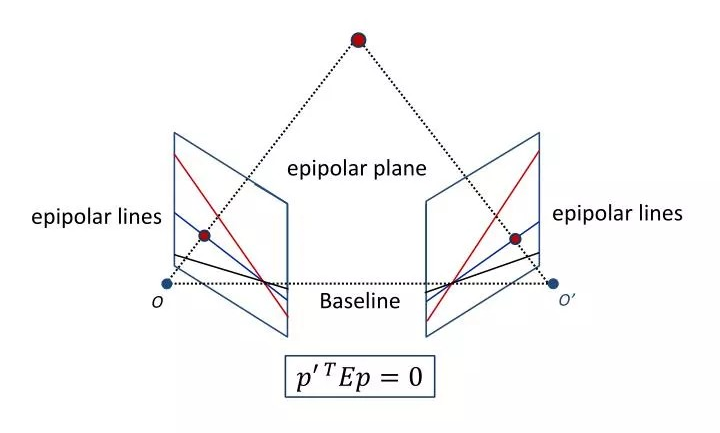
\includegraphics[width=1\linewidth]{images/l12-epipolar.png}
% 3. \textbf{Epipolar Plane:} The plane formed by a 3D point \(X\) and the optical centers of both cameras. Each epipolar plane intersects the two image planes along corresponding epipolar lines. \\

% 4. \textbf{Epipolar Lines:} 
%    - For a point \(p\) in the first image, the corresponding point \(p'\) in the second image must lie on its epipolar line.
%    - This reduces the matching search from 2D to 1D along the epipolar line, greatly simplifying stereo matching. \\

\subsection*{Fundamental and Essential Matrices:}
1. \textbf{Fundamental Matrix \(F\)} relates corresponding points in two \textit{uncalibrated} images, singular(r=2), deg free=7:
     \[
     \mathbf{{p'}}^T F \mathbf{{p}} = 0.
     \]
     It maps a point \(p\) in the first image to its epipolar line in the second image. \\
2. \textbf{Essential Matrix \(E\)} is a special case for \textit{calibrated} cameras:
     \[
     E = [t_x] R,
     \]
     \(R\) : rotation matrix, \([t_x]\) : skew-symmetric matrix representing translation. \\

3. \textbf{Epipolar Constraint (Calibrated Case):}
    With known intrinsic matrices \(K_1\) and \(K_2\), the projection matrices are:
     \[
     M_1 = K_1 [I \mid 0], \quad M_2 = K_2 [R \mid t].
     \]
   % - Given a point \(p\) in the first image, its corresponding point \(p'\) in the second image satisfies:
     \[
     \mathbf{\hat{p'}}^T E \mathbf{\hat{p}} = 0.
     \]
\subsection*{Estimating the Fundamental Matrix}
% 1. \textbf{Objective:} The fundamental matrix \( F \) relates corresponding points between two views in uncalibrated stereo systems. It maps a point \( p \) in the first image to its epipolar line in the second image:
%    \[
%    \mathbf{p'}^T F \mathbf{p} = 0,
%    \]
%    where \( \mathbf{p} = (u, v, 1)^T \) and \( \mathbf{p'} = (u', v', 1)^T \) are corresponding points in homogeneous coordinates. \\

% 2. \textbf{Fundamental Matrix Representation:}
%    - \( F \) is a \( 3 \times 3 \) matrix that encodes the epipolar geometry between two views.
%    - It is rank-deficient (rank 2) and has 7 degrees of freedom. \\

1. \textbf{Linear Estimation of \( F \):}
   From the epipolar constraint and Stacking:

     \[
     u' u f_{11} + u' v f_{12} + u' f_{13} + v' u f_{21} 
     % + v' f_{23} + u f_{31} + v f_{32} + f_{33} = 0.
     \]
     \[
     % u' u f_{11} + u' v f_{12} + u' f_{13} + v' u f_{21} + v' v f_{22} 
     + v' v f_{22}  + v' f_{23} + u f_{31} + v f_{32} + f_{33} = 0.
     \]
     \[
     A \mathbf{f} = 0,
     \]
     where \( A \) is an \( 8 \times 9 \) matrix constructed from the point correspondences, and \( \mathbf{f} \) is the 9-vector representing the entries of \( F \). \\

2. \textbf{Eight-Point Algorithm:}
   - Solve the system \( A \mathbf{f} = 0 \) using Singular Value Decomposition (SVD) to estimate \( F \).
   - \( F \) rank 2, set the smallest singular value of \( F \) to zero. \\

3. \textbf{Normalization:}
   - For better numerical stability:
     \[
     \mathbf{p} \rightarrow \frac{\mathbf{p}}{\|\mathbf{p}\|}, \quad \mathbf{p'} \rightarrow \frac{\mathbf{p'}}{\|\mathbf{p'}\|}.
     \]
   - After the estimation, the fundamental matrix should be denormalized. \\

4. \textbf{RANSAC for Robust Estimation:}
   % - Since real data often includes noise and outliers, the RANSAC algorithm is often used to robustly estimate \( F \).
   - RANSAC randomly samples minimal sets of correspondences (8) to estimate \( F \) and selects the solution that maximizes the number of inliers (pts that satisfy the epipolar constraint within a threshold). \\


% 8. \textbf{Applications of Epipolar Geometry:}
%    - Used in **stereo vision** to recover depth by matching corresponding points along epipolar lines.
%    - Essential for **3D reconstruction**, structure from motion, and camera calibration.

\section{Depth from Stereo \& Structure from Motion}

\subsection*{Depth from Stereo:}
1. \textbf{Goal:} Recover depth by finding corresponding points in two images (stereo matching). Depth is inversely related to disparity.
   
2. \textbf{Disparity:} 
   - Disparity \( d = x - x' \), where \( x \) and \( x' \) are corresponding image coordinates in two views.
   % - Depth \( z \) is related to disparity as:
     \[
     depth = \frac{f B}{d},
     \]
     \(d\): depth, \( f \) : focal length, \( B \) : baseline distance between cameras.

3. \textbf{Stereo Matching Algorithm:}
   - For each pixel in imgA, find corresponding epipolar line in imgB.
   - Search along epipolar line and select  best match based on a similarity measure (e.g., SSD, normalized correlation).
   - Triangulate to obtain depth.

4. \textbf{Rectification:} Reproject image planes onto a common plane to transform epipolar lines into horizontal scanlines, simplifying correspondence search.

5. \textbf{Basic Challenges:}
   - Textureless regions: Hard to find unique correspondences.
   - Repeated patterns: Ambiguity in matching points.
   - Specular surfaces: Appearance changes with viewpoint.

\subsection*{Structure from Motion (SfM):}
1. \textbf{Goal:} Recover 3D structure and camera motion from multiple views.

2. \textbf{Projection Model:}
   - For a 3D point \( X_j \) and camera \( M_i \), the image point \( p_{ij} \) is given by:
     \[
     p_{ij} \equiv M_i X_j, \quad p_{ij} = M_i X_j.
     \]
   - \( M_i = K_i [R_i | t_i] \), \( K_i \) : intrinsic matrix,  \( R_i, t_i \): extrinsic parameters.

3. \textbf{Ambiguities in SfM:}
   - \textbf{Scale ambiguity:} Cannot determine absolute scale from motion alone.
   - \textbf{Projective ambiguity:} Without constraints, reconstruction is only determined up to a projective transformation.
   - \textbf{Affine ambiguity:} If parallel lines are known, ambiguity reduces to affine. Additional constraints can reduce ambiguity to similarity.

4. \textbf{Affine Structure from Motion:}
   - Use affine cameras for a simplified SfM approach. For \( m \) cameras and \( n \) points:
     \[
     p_{ij} \equiv A_i X_j + b_i,
     \]
      \( A_i \) : affine projection matrix. \( b_i \) :  translation.\\
   - Factorize the measurement matrix to recover motion and structure:
     \[
     D = \begin{bmatrix} A_1 \\ \vdots \\ A_m \end{bmatrix} \begin{bmatrix} X_1 & \dots & X_n \end{bmatrix}.
     \]

5. \textbf{Triangulation in SfM:}
   - Estimate the 3D points \( X_j \) by minimizing the reprojection error across all views:
     \[
     \sum_i \| p_{ij} - M_i X_j \|^2.
     \]
   - Use optimization techniques such as bundle adjustment to refine the structure and motion estimates.

% \subsection*{Summary:}
% - \textbf{Depth from Stereo:} Find correspondences between two images, compute disparity, and infer depth.
% - \textbf{Structure from Motion:} Recover 3D structure and camera motion from multiple views, with challenges in handling ambiguities.

\end{multicols*}
\end{document}